\documentclass[conference]{IEEEtran}
\IEEEoverridecommandlockouts
\usepackage{cite}
\usepackage{amsmath,amssymb,amsfonts}
\usepackage{graphicx}
\usepackage{booktabs}
\usepackage{url}
\usepackage{placeins}
\hyphenation{XCCNet Kermany Grad-CAM}
\begin{document}
\title{Reproducing XCCNet for Pediatric Pneumonia: Focal Loss Does Not Help, and the Lung Mask Hurts}
\author{\IEEEauthorblockN{Kartik Yadav, Gangadhar Yadav, and Sahil Sarawgi}}
\maketitle

\begin{abstract}
We reproduce XCCNet, a dilated CNN joined with a frozen CLIP encoder, for pneumonia-versus-normal classification on the Kermany pediatric chest X-rays. The code is not public, so we rebuild the model from the paper without its GAN and rib-suppression stages. On the paper's stratified 80/10/10 split, our first run reaches 94.87\% test accuracy. The paper reports 97.18\% for the same setting, but its own precision and recall imply 94.84\% at our class mix. Most errors are normal films called pneumonia. Before coding, we predicted that focal loss would raise specificity from 85\% to 88--91\%. Over three seeds it lowered specificity to 79.1\% and left AUC unchanged (0.975 vs 0.978). With the threshold tuned on validation, both losses reach the same specificity. Focal loss only rescaled the scores. A second ablation removes the lung mask. Against our prediction, accuracy rises from 92.7\% to 95.8\% and AUC from 0.978 to 0.993. Grad-CAM and mask coverage suggest the adult-trained mask cuts off lung in child films. We make no clinical claim.
\end{abstract}
\begin{IEEEkeywords}
Pediatric pneumonia, chest X-ray, reproduction, focal loss, lung segmentation, Grad-CAM.
\end{IEEEkeywords}

\section{Introduction}
Pneumonia is a leading cause of death in children under five. A chest X-ray is the usual first test, and reading it takes a trained radiologist. Kermany \textit{et al.} released 5{,}856 pediatric chest X-rays from Guangzhou in 2018~\cite{kermany2018}. Many deep learning papers report pneumonia-versus-normal accuracy on this set, from 86\% to above 99\%.

These numbers are hard to compare. Papers that keep the official 624-patient test report 86\% to 95\%~\cite{kermany2018,rajaraman2018,salehi2021,ayan2021}. Papers that pool the data and draw an 80/10/10 split report about 99\%~\cite{raghaw2024,choudhury2026}. Most papers report accuracy, precision, recall, and F1. Few report specificity or AUC. Pneumonia outnumbers normal about 3 to 1, so accuracy can hide errors on the normal class.

We reproduce XCCNet~\cite{raghaw2024} on the paper's split and add specificity and AUC. Our model makes most of its errors on normal films. We test one change, focal loss~\cite{lin2017}, and stated the prediction before writing code. To check whether a gain is more than a threshold shift, we compare focal loss against the baseline with a threshold tuned on validation. We also run one ablation without the lung mask.

Our contributions are: (1) a reimplementation of XCCNet without its GAN and rib suppressor, with specificity and AUC; (2) a check of the paper's accuracy against its own precision and recall; (3) a pre-stated, tested focal-loss hypothesis with a threshold control, a lung-mask ablation, and a failure analysis.

\section{Related Work}
Kermany \textit{et al.} froze an ImageNet Inception V3 and reached 92.8\% accuracy and 96.8\% AUC on the 624-patient test~\cite{kermany2018}. Rajaraman \textit{et al.} cropped the lungs with an atlas and raised accuracy to 96.2\%~\cite{rajaraman2018}. Stephen \textit{et al.} trained a small CNN from scratch~\cite{stephen2019}. Rahman \textit{et al.} compared four ImageNet networks and found DenseNet201 best~\cite{rahman2020}. Salehi \textit{et al.} used SMOTE and warned that one child's films can fall in both train and test~\cite{salehi2021}. Ayan \textit{et al.} and Kundu \textit{et al.} used ensembles; Kundu's accuracy fell from 98.81\% to 86.95\% on RSNA films~\cite{ayan2021,kundu2021}. Chauhan \textit{et al.} used class weights in a 388k-parameter network~\cite{chauhan2025}. Choudhury fine-tuned ResNet50 to 99.43\% on an 80/10/10 split~\cite{choudhury2026}. XCCNet joins a dilated CNN with CLIP~\cite{radford2021}, a contrastive term, a GAN for extra normal films, and rib suppression, and reports 99.76\%~\cite{raghaw2024}. None of these ten papers uses focal loss.

\section{Method}
\subsection{Baseline}
The spatial branch has five dilated $3\times3$ convolution blocks (dilation 2, 32 to 512 filters), each with batch norm, ReLU, $2\times2$ pooling, and dropout 0.1. A $1\times1$ convolution maps the final $8\times8\times512$ map to 2{,}304 values. The global branch is a frozen CLIP ViT-B/32~\cite{radford2021} with a 512-dimensional output. The two vectors are joined (2{,}816 values) and passed to a two-layer head with a sigmoid output. The loss is the paper's Eq.~15:
\begin{equation}
L = \phi\,L_{\text{con}} + (1-\phi)\,L_{\text{cls}} + \lambda\,L_{1},\qquad \phi = \tfrac{1}{e+1},
\end{equation}
where $L_{\text{con}}$ is a symmetric InfoNCE loss between the two branches, $L_{\text{cls}}$ is binary cross-entropy, and $e$ is the epoch. Images are resized to $256\times256$ and enhanced with CLAHE (clip 2.0, $8\times8$ tiles). A lung mask from the public ChestX-Det PSPNet~\cite{cohen2022} sets pixels outside the lungs to zero, because Kermany has no masks for the paper's ResUNet++. A weighted sampler balances the two classes in each batch. Training uses Adam at $10^{-4}$, batch 16, a $0.3\times$ learning-rate drop on a validation plateau, and early stopping with patience 5.

\textit{Not reproduced.} The GAN has no layer sizes or weights in the paper. Rib suppression needs paired bone-suppressed images, which Kermany does not have.

\subsection{Our change: focal loss}
We replace binary cross-entropy in $L_{\text{cls}}$ with focal loss~\cite{lin2017}:
\begin{equation}
L_{\text{focal}} = -(1-p_t)^{\gamma}\log p_t,\qquad \gamma = 2,
\end{equation}
where $p_t$ is the predicted probability of the true class. A film the model already gets right with $p_t = 0.95$ keeps only $0.0025$ of its loss. Nothing else changes.

\textit{Hypothesis and prediction (stated before coding).} Most errors are normal films that look a little like pneumonia. Focal loss moves gradient toward hard films, so specificity should rise from 85\% to 88--91\%, sensitivity should stay within 1 point, and AUC should stay within $\pm0.005$. We noted one risk: the sampler already balances the classes.

\subsection{Controls}
Row A$'$ uses the baseline's saved scores with the threshold that maximises sensitivity + specificity on validation (Youden's J). It needs no training. If focal loss beats A$'$, it changed what the model learned. If not, it only moved the threshold. Row C turns the lung mask off. We predicted accuracy would fall by 0.5--2 points, because without the mask the model can use text markers and edges.

\section{Experiments}
\textit{Data.} Kaggle mirror of Kermany~\cite{kermany2018}: 1{,}583 normal and 4{,}273 pneumonia films, pooled and split 80/10/10 per class with seed 42. Train 4{,}686, validation 585, test 585 (427 pneumonia, 158 normal). Every run uses the same split.

\textit{Protocol.} Each row is trained with three seeds (42, 1, 2). Validation accuracy picks the epoch. The test set is read once per run. Pneumonia is the positive class: sensitivity is pneumonia recall and specificity is normal recall. Hardware is one free Colab T4. A run takes 3--10 minutes once images are cached.

\begin{table}[t]
\caption{Test results, mean $\pm$ std over three seeds. FP and FN are mean counts out of 158 normal and 427 pneumonia films.}
\label{tab:ablation}
\centering
\footnotesize
\setlength{\tabcolsep}{3pt}
\resizebox{\columnwidth}{!}{%
\begin{tabular}{@{}lccccc@{}}
\toprule
Row & Acc \% & Sens \% & Spec \% & AUC & FP / FN \\
\midrule
A: baseline & 92.71$\pm$0.55 & 95.32$\pm$1.87 & 85.65$\pm$3.25 & .978$\pm$.004 & 22.7 / 20.0 \\
A$'$: A, val threshold & 92.42$\pm$0.69 & 93.29$\pm$1.51 & 90.08$\pm$2.22 & .978$\pm$.004 & 15.7 / 28.7 \\
B: focal $\gamma{=}2$ & 91.68$\pm$0.39 & 96.33$\pm$1.08 & 79.11$\pm$2.53 & .975$\pm$.003 & 33.0 / 15.7 \\
C: no lung mask & 95.78$\pm$0.26 & 97.97$\pm$0.36 & 89.87$\pm$1.90 & .993$\pm$.001 & 16.0 / \phantom{0}8.7 \\
\bottomrule
\end{tabular}}
\end{table}

\begin{table}[t]
\caption{Prediction versus result.}
\label{tab:pred}
\centering
\footnotesize
\begin{tabular}{@{}lll@{}}
\toprule
Row & Predicted & Result \\
\midrule
A & AUC 0.97--0.99 & 0.978 (correct) \\
A$'$ & Spec $+$2--5, sens $-$1 & Spec $+$4.4, sens $-$2.0 \\
B & Spec 88--91\%, AUC $\pm$.005 & Spec 79.1\% (wrong), AUC $-$.003 \\
C & Acc $-$0.5 to $-$2 & Acc $+$3.1 (wrong) \\
\bottomrule
\end{tabular}
\end{table}

\section{Results and Discussion}
\subsection{Focal loss}
Table~\ref{tab:ablation} shows that focal loss lowered specificity by 6.5 points and raised sensitivity by 1.0 point. AUC did not change beyond seed noise. Our prediction was wrong on specificity and right on AUC (Table~\ref{tab:pred}).

The scores explain this. With cross-entropy, 78\% of test films score below 0.1 or above 0.9. With focal loss, 35\% do. The median normal film moves from 0.08 to 0.35. Focal loss stops pushing easy films toward 0 or 1, so the scores bunch toward the middle. The sampler shows the model equal numbers of each class, and pneumonia films still carry more of the remaining loss, so more normal films cross 0.5. When the threshold is tuned on validation for both models, both reach 90.1\% specificity, and focal loss has slightly lower sensitivity (92.4\% vs 93.3\%). So B does not beat A$'$. Focal loss rescaled the scores. It did not change how the model ranks films. The risk we noted came true: the sampler had already handled the imbalance.

\subsection{Lung mask}
Removing the mask raised every metric, against our prediction. Accuracy rose by 3.1 points, false negatives fell from 20.0 to 8.7, and seed spread shrank. The mask model was trained on adult films at $512\times512$, and we run it on child films at $256\times256$. In seed 42 of row A, normal films in the quarter with the smallest masks have a 23.4\% error rate, against 14.4\% for the rest. Fig.~\ref{fig:failA} shows normal films with a missing lower lobe or most of one lung, scored 0.93--0.98. Grad-CAM often marks the mask edge, the diaphragm line, and the black area below the lungs.

A higher score without the mask does not prove a better model. Without the mask the model can also use the ``R'' marker, film borders, and body size. Some row C failures have Grad-CAM hot spots in the lower corners of the film (Fig.~\ref{fig:failC}). One hospital's data cannot separate real lung findings from such shortcuts.

\begin{figure*}[t]
\centering
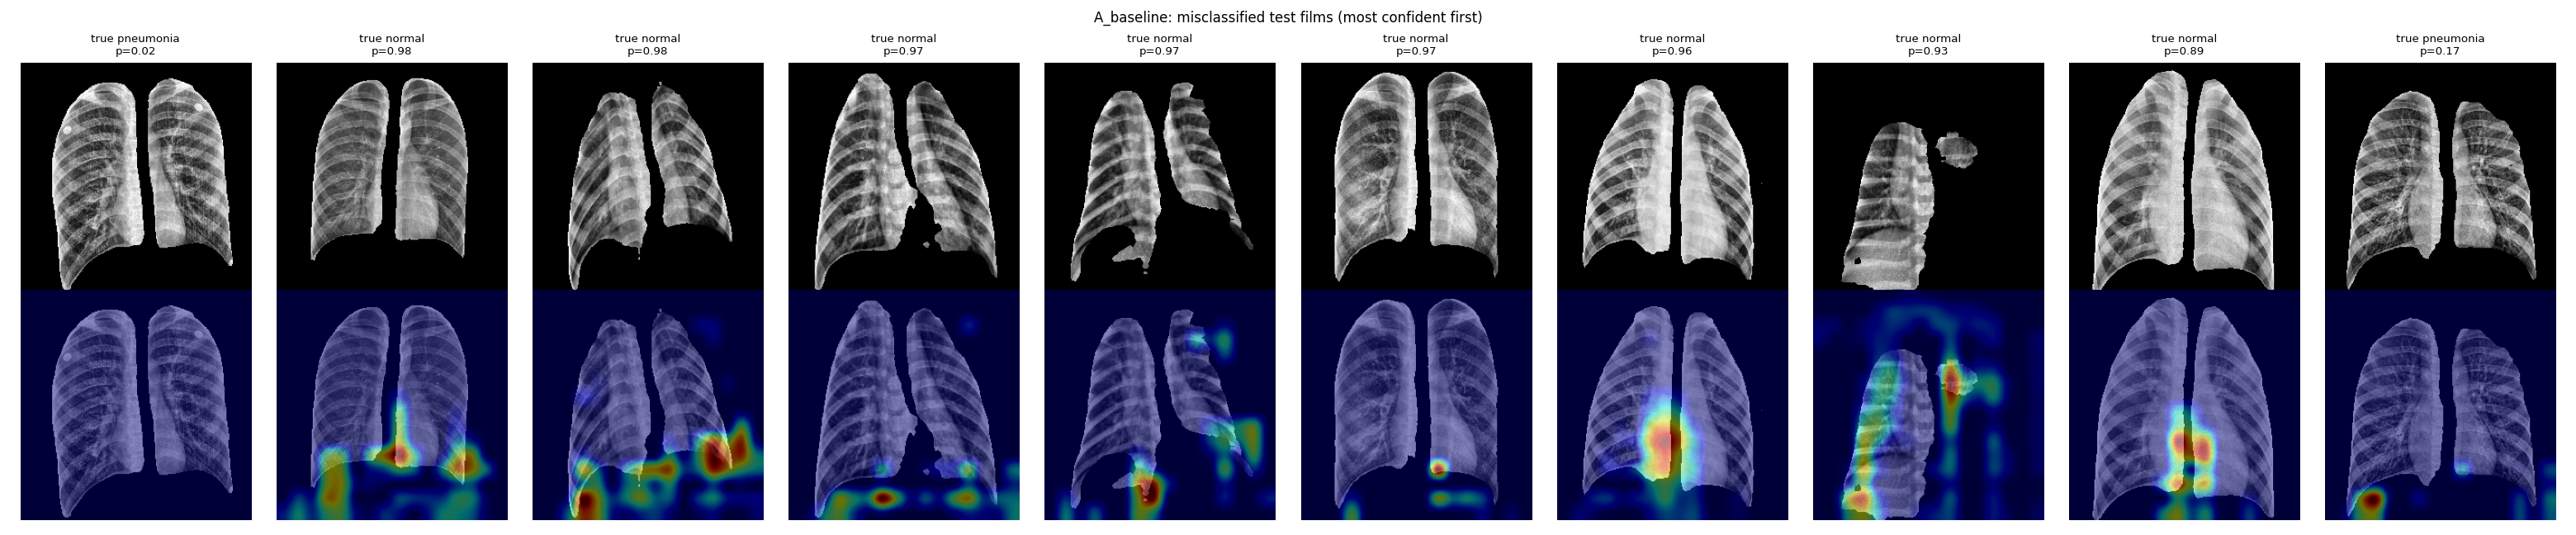
\includegraphics[width=\textwidth]{figures/failures_A.png}
\caption{Row A (baseline, seed 42): the ten most confident test errors. Top: input after CLAHE and the lung mask, with true label and predicted probability. Bottom: Grad-CAM. Several normal films lose part of the lung to the mask.}
\label{fig:failA}
\end{figure*}

\begin{figure*}[t]
\centering
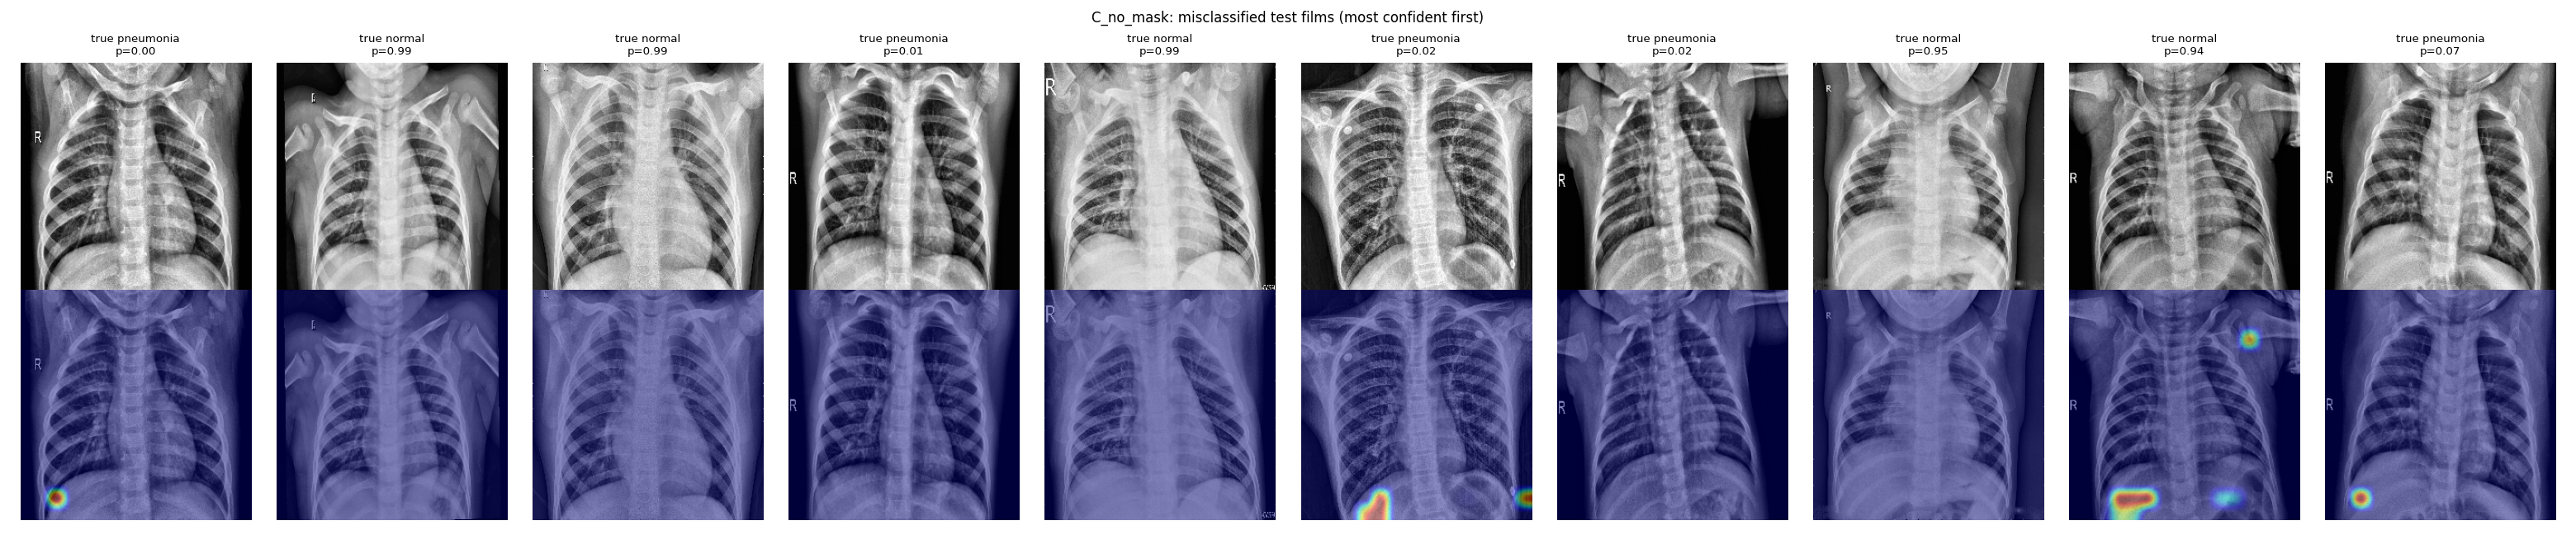
\includegraphics[width=\textwidth]{figures/failures_C.png}
\caption{Row C (no lung mask, seed 42): the ten most confident test errors. Some Grad-CAM hot spots fall in the lower corners, outside the lungs.}
\label{fig:failC}
\end{figure*}

\subsection{Failure analysis}
In every row the most common error is a normal film called pneumonia (Fig.~\ref{fig:cm}). Kaggle file names label pneumonia as bacterial or viral. We did not train on this split, but counting errors by subtype gives, for row A, recall of 85.7\% on normal, 96.5\% on bacterial, and 93.4\% on viral films. Viral pneumonia is a faint haze across both lungs and is closer to a normal film than a dense bacterial patch. Ayan \textit{et al.} report the same weak viral class~\cite{ayan2021}. The most confident miss in row A (p = 0.02) is a pneumonia film whose lungs look clear after CLAHE. It may be very mild or mislabelled. We cannot tell without a radiologist.

\begin{figure}[t]
\centering
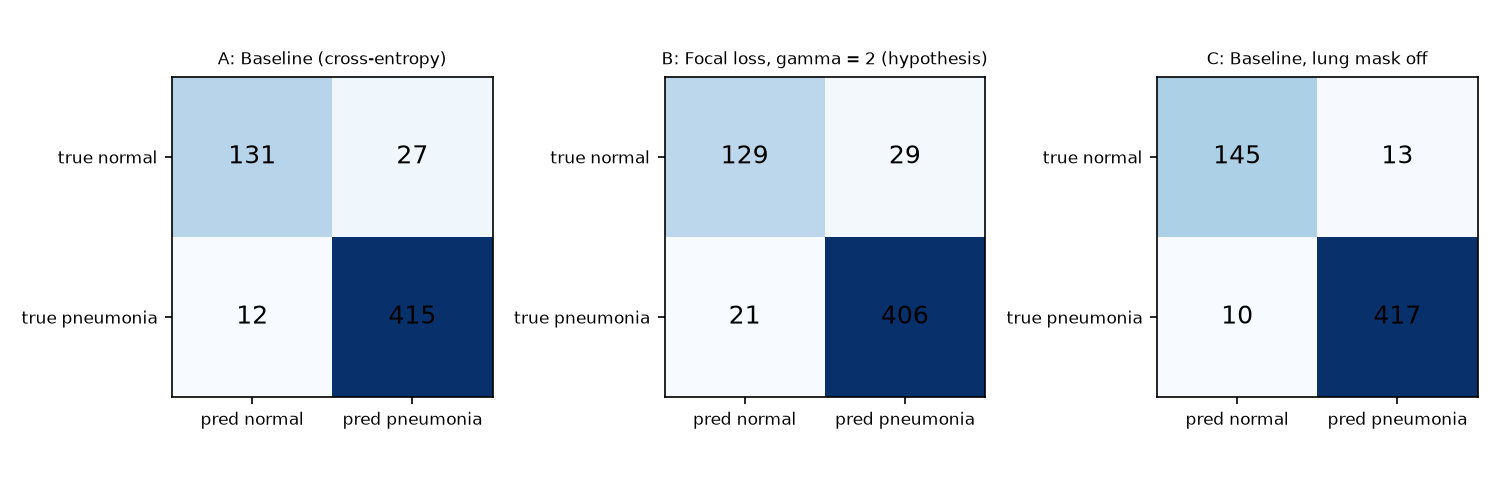
\includegraphics[width=\columnwidth]{figures/confusion_matrices.png}
\caption{Confusion matrices at threshold 0.5, seed 42.}
\label{fig:cm}
\end{figure}

\begin{figure}[t]
\centering
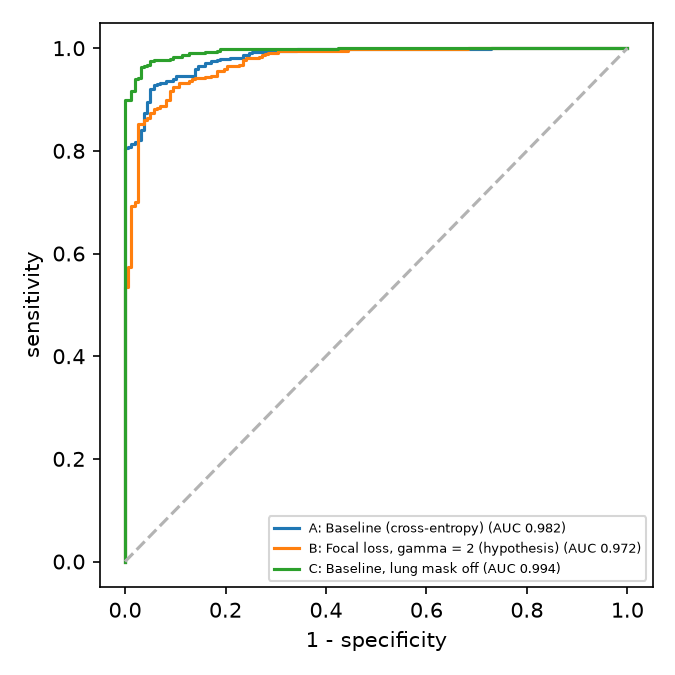
\includegraphics[width=0.8\columnwidth]{figures/roc_curves.png}
\caption{Test ROC curves, seed 42.}
\label{fig:roc}
\end{figure}

\subsection{Reproduction gap}
The paper reports 97.18\% accuracy, 94.52\% precision, and 98.65\% recall for its setting without the GAN~\cite{raghaw2024}. At our test mix of 427 pneumonia and 158 normal films, that precision and recall give 94.84\% accuracy. Our first run reached 94.87\%. The paper's 97.18\% only fits a test set with a different class mix. In that first run, the file order depended on the disk, so the split could not be rebuilt. We sorted the files before splitting, and the baseline under the fixed split averages 92.71\%. Part of the 2-point drop is which films land in the test set. Between seeds, specificity moves from 82.9\% to 89.2\%, so a one-seed comparison between rows would not be reliable. The other differences from the paper are the missing GAN and rib suppressor, the stand-in lung mask, and the learning rate ($10^{-4}$ instead of $10^{-6}$, because our CNN trains from scratch).

\section{Limitations}
All films come from one hospital, and the children are aged 1 to 5. There is no external test, so we cannot say whether row C relies on lung findings or on shortcuts. We use the paper's pooled 80/10/10 split, not the official 624-patient test, and one child's films may fall in both train and test~\cite{salehi2021}. We ran three seeds on one split. Early stopping on validation accuracy picked epoch 2 in several runs, and a different rule could change the numbers. The lung mask is a stand-in for the paper's ResUNet++. We make no clinical claim.

\section{Conclusion}
We rebuilt XCCNet without its GAN and rib suppressor and matched the accuracy implied by the paper's own precision and recall. Our pre-stated hypothesis, that focal loss would fix false positives on normal films, was wrong: it rescaled the scores without changing AUC, and a tuned threshold did as well. Removing the adult-trained lung mask raised AUC from 0.978 to 0.993, which points to the mask cutting lung in child films, though shortcuts outside the lungs may also play a part. Next steps are a mask trained on pediatric films, the official 624-patient test, and a test on another hospital's films.

\begin{thebibliography}{00}
\bibitem{kermany2018} D.~S. Kermany, M.~Goldbaum, W.~Cai \textit{et al.}, ``Identifying medical diagnoses and treatable diseases by image-based deep learning,'' \textit{Cell}, vol.~172, no.~5, pp.~1122--1131.e2, 2018.
\bibitem{rajaraman2018} S.~Rajaraman, S.~Candemir, I.~Kim, G.~Thoma, and S.~Antani, ``Visualization and interpretation of convolutional neural network predictions in detecting pneumonia in pediatric chest radiographs,'' \textit{Appl.\ Sci.}, vol.~8, no.~10, p.~1715, 2018.
\bibitem{stephen2019} O.~Stephen, M.~Sain, U.~J. Maduh, and D.-U. Jeong, ``An efficient deep learning approach to pneumonia classification in healthcare,'' \textit{J.\ Healthc.\ Eng.}, vol.~2019, p.~4180949, 2019.
\bibitem{rahman2020} T.~Rahman, M.~E.~H. Chowdhury \textit{et al.}, ``Transfer learning with deep convolutional neural network (CNN) for pneumonia detection using chest X-ray,'' arXiv:2004.06578, 2020.
\bibitem{salehi2021} M.~Salehi, R.~Mohammadi, H.~Ghaffari, N.~Sadighi, and R.~Reiazi, ``Automated detection of pneumonia cases using deep transfer learning with paediatric chest X-ray images,'' \textit{Br.\ J.\ Radiol.}, vol.~94, p.~20201263, 2021.
\bibitem{ayan2021} E.~Ayan, B.~Karabulut, and H.~M. \"Unver, ``Diagnosis of pediatric pneumonia with ensemble of deep convolutional neural networks in chest X-ray images,'' \textit{Arab.\ J.\ Sci.\ Eng.}, vol.~47, pp.~2123--2139, 2021.
\bibitem{kundu2021} R.~Kundu, R.~Das, Z.~W. Geem, G.-T. Han, and R.~Sarkar, ``Pneumonia detection in chest X-ray images using an ensemble of deep learning models,'' \textit{PLoS One}, vol.~16, no.~9, p.~e0256630, 2021.
\bibitem{raghaw2024} C.~S. Raghaw, P.~S. Bhore, M.~Z.~U. Rehman, and N.~Kumar, ``An explainable contrastive-based dilated convolutional network with transformer for pediatric pneumonia detection,'' arXiv:2410.16143, 2024.
\bibitem{chauhan2025} N.~Chauhan, P.~K. Gupta, and F.~Doja, ``LightPneumoNet: Lightweight pneumonia classifier,'' arXiv:2510.11232, 2025.
\bibitem{choudhury2026} A.~R. Choudhury, ``Pediatric pneumonia detection from chest X-rays: A comparative study of transfer learning and custom CNNs,'' arXiv:2601.00837, 2026.
\bibitem{lin2017} T.-Y. Lin, P.~Goyal, R.~Girshick, K.~He, and P.~Doll\'ar, ``Focal loss for dense object detection,'' in \textit{Proc.\ IEEE ICCV}, 2017, pp.~2980--2988.
\bibitem{radford2021} A.~Radford, J.~W. Kim, C.~Hallacy \textit{et al.}, ``Learning transferable visual models from natural language supervision,'' in \textit{Proc.\ ICML}, 2021, pp.~8748--8763.
\bibitem{cohen2022} J.~P. Cohen, J.~D. Viviano, P.~Bertin \textit{et al.}, ``TorchXRayVision: A library of chest X-ray datasets and models,'' in \textit{Proc.\ MIDL}, 2022, pp.~231--249.
\end{thebibliography}
\end{document}
